% Options for packages loaded elsewhere
\PassOptionsToPackage{unicode}{hyperref}
\PassOptionsToPackage{hyphens}{url}
\PassOptionsToPackage{dvipsnames,svgnames,x11names}{xcolor}
%
\documentclass[
  letterpaper,
  DIV=11,
  numbers=noendperiod]{scrartcl}

\usepackage{amsmath,amssymb}
\usepackage{lmodern}
\usepackage{iftex}
\ifPDFTeX
  \usepackage[T1]{fontenc}
  \usepackage[utf8]{inputenc}
  \usepackage{textcomp} % provide euro and other symbols
\else % if luatex or xetex
  \usepackage{unicode-math}
  \defaultfontfeatures{Scale=MatchLowercase}
  \defaultfontfeatures[\rmfamily]{Ligatures=TeX,Scale=1}
\fi
% Use upquote if available, for straight quotes in verbatim environments
\IfFileExists{upquote.sty}{\usepackage{upquote}}{}
\IfFileExists{microtype.sty}{% use microtype if available
  \usepackage[]{microtype}
  \UseMicrotypeSet[protrusion]{basicmath} % disable protrusion for tt fonts
}{}
\makeatletter
\@ifundefined{KOMAClassName}{% if non-KOMA class
  \IfFileExists{parskip.sty}{%
    \usepackage{parskip}
  }{% else
    \setlength{\parindent}{0pt}
    \setlength{\parskip}{6pt plus 2pt minus 1pt}}
}{% if KOMA class
  \KOMAoptions{parskip=half}}
\makeatother
\usepackage{xcolor}
\setlength{\emergencystretch}{3em} % prevent overfull lines
\setcounter{secnumdepth}{-\maxdimen} % remove section numbering
% Make \paragraph and \subparagraph free-standing
\ifx\paragraph\undefined\else
  \let\oldparagraph\paragraph
  \renewcommand{\paragraph}[1]{\oldparagraph{#1}\mbox{}}
\fi
\ifx\subparagraph\undefined\else
  \let\oldsubparagraph\subparagraph
  \renewcommand{\subparagraph}[1]{\oldsubparagraph{#1}\mbox{}}
\fi

\usepackage{color}
\usepackage{fancyvrb}
\newcommand{\VerbBar}{|}
\newcommand{\VERB}{\Verb[commandchars=\\\{\}]}
\DefineVerbatimEnvironment{Highlighting}{Verbatim}{commandchars=\\\{\}}
% Add ',fontsize=\small' for more characters per line
\usepackage{framed}
\definecolor{shadecolor}{RGB}{241,243,245}
\newenvironment{Shaded}{\begin{snugshade}}{\end{snugshade}}
\newcommand{\AlertTok}[1]{\textcolor[rgb]{0.68,0.00,0.00}{#1}}
\newcommand{\AnnotationTok}[1]{\textcolor[rgb]{0.37,0.37,0.37}{#1}}
\newcommand{\AttributeTok}[1]{\textcolor[rgb]{0.40,0.45,0.13}{#1}}
\newcommand{\BaseNTok}[1]{\textcolor[rgb]{0.68,0.00,0.00}{#1}}
\newcommand{\BuiltInTok}[1]{\textcolor[rgb]{0.00,0.23,0.31}{#1}}
\newcommand{\CharTok}[1]{\textcolor[rgb]{0.13,0.47,0.30}{#1}}
\newcommand{\CommentTok}[1]{\textcolor[rgb]{0.37,0.37,0.37}{#1}}
\newcommand{\CommentVarTok}[1]{\textcolor[rgb]{0.37,0.37,0.37}{\textit{#1}}}
\newcommand{\ConstantTok}[1]{\textcolor[rgb]{0.56,0.35,0.01}{#1}}
\newcommand{\ControlFlowTok}[1]{\textcolor[rgb]{0.00,0.23,0.31}{#1}}
\newcommand{\DataTypeTok}[1]{\textcolor[rgb]{0.68,0.00,0.00}{#1}}
\newcommand{\DecValTok}[1]{\textcolor[rgb]{0.68,0.00,0.00}{#1}}
\newcommand{\DocumentationTok}[1]{\textcolor[rgb]{0.37,0.37,0.37}{\textit{#1}}}
\newcommand{\ErrorTok}[1]{\textcolor[rgb]{0.68,0.00,0.00}{#1}}
\newcommand{\ExtensionTok}[1]{\textcolor[rgb]{0.00,0.23,0.31}{#1}}
\newcommand{\FloatTok}[1]{\textcolor[rgb]{0.68,0.00,0.00}{#1}}
\newcommand{\FunctionTok}[1]{\textcolor[rgb]{0.28,0.35,0.67}{#1}}
\newcommand{\ImportTok}[1]{\textcolor[rgb]{0.00,0.46,0.62}{#1}}
\newcommand{\InformationTok}[1]{\textcolor[rgb]{0.37,0.37,0.37}{#1}}
\newcommand{\KeywordTok}[1]{\textcolor[rgb]{0.00,0.23,0.31}{#1}}
\newcommand{\NormalTok}[1]{\textcolor[rgb]{0.00,0.23,0.31}{#1}}
\newcommand{\OperatorTok}[1]{\textcolor[rgb]{0.37,0.37,0.37}{#1}}
\newcommand{\OtherTok}[1]{\textcolor[rgb]{0.00,0.23,0.31}{#1}}
\newcommand{\PreprocessorTok}[1]{\textcolor[rgb]{0.68,0.00,0.00}{#1}}
\newcommand{\RegionMarkerTok}[1]{\textcolor[rgb]{0.00,0.23,0.31}{#1}}
\newcommand{\SpecialCharTok}[1]{\textcolor[rgb]{0.37,0.37,0.37}{#1}}
\newcommand{\SpecialStringTok}[1]{\textcolor[rgb]{0.13,0.47,0.30}{#1}}
\newcommand{\StringTok}[1]{\textcolor[rgb]{0.13,0.47,0.30}{#1}}
\newcommand{\VariableTok}[1]{\textcolor[rgb]{0.07,0.07,0.07}{#1}}
\newcommand{\VerbatimStringTok}[1]{\textcolor[rgb]{0.13,0.47,0.30}{#1}}
\newcommand{\WarningTok}[1]{\textcolor[rgb]{0.37,0.37,0.37}{\textit{#1}}}

\providecommand{\tightlist}{%
  \setlength{\itemsep}{0pt}\setlength{\parskip}{0pt}}\usepackage{longtable,booktabs,array}
\usepackage{calc} % for calculating minipage widths
% Correct order of tables after \paragraph or \subparagraph
\usepackage{etoolbox}
\makeatletter
\patchcmd\longtable{\par}{\if@noskipsec\mbox{}\fi\par}{}{}
\makeatother
% Allow footnotes in longtable head/foot
\IfFileExists{footnotehyper.sty}{\usepackage{footnotehyper}}{\usepackage{footnote}}
\makesavenoteenv{longtable}
\usepackage{graphicx}
\makeatletter
\def\maxwidth{\ifdim\Gin@nat@width>\linewidth\linewidth\else\Gin@nat@width\fi}
\def\maxheight{\ifdim\Gin@nat@height>\textheight\textheight\else\Gin@nat@height\fi}
\makeatother
% Scale images if necessary, so that they will not overflow the page
% margins by default, and it is still possible to overwrite the defaults
% using explicit options in \includegraphics[width, height, ...]{}
\setkeys{Gin}{width=\maxwidth,height=\maxheight,keepaspectratio}
% Set default figure placement to htbp
\makeatletter
\def\fps@figure{htbp}
\makeatother

\KOMAoption{captions}{tableheading}
\makeatletter
\makeatother
\makeatletter
\makeatother
\makeatletter
\@ifpackageloaded{caption}{}{\usepackage{caption}}
\AtBeginDocument{%
\ifdefined\contentsname
  \renewcommand*\contentsname{Table of contents}
\else
  \newcommand\contentsname{Table of contents}
\fi
\ifdefined\listfigurename
  \renewcommand*\listfigurename{List of Figures}
\else
  \newcommand\listfigurename{List of Figures}
\fi
\ifdefined\listtablename
  \renewcommand*\listtablename{List of Tables}
\else
  \newcommand\listtablename{List of Tables}
\fi
\ifdefined\figurename
  \renewcommand*\figurename{Figure}
\else
  \newcommand\figurename{Figure}
\fi
\ifdefined\tablename
  \renewcommand*\tablename{Table}
\else
  \newcommand\tablename{Table}
\fi
}
\@ifpackageloaded{float}{}{\usepackage{float}}
\floatstyle{ruled}
\@ifundefined{c@chapter}{\newfloat{codelisting}{h}{lop}}{\newfloat{codelisting}{h}{lop}[chapter]}
\floatname{codelisting}{Listing}
\newcommand*\listoflistings{\listof{codelisting}{List of Listings}}
\makeatother
\makeatletter
\@ifpackageloaded{caption}{}{\usepackage{caption}}
\@ifpackageloaded{subcaption}{}{\usepackage{subcaption}}
\makeatother
\makeatletter
\@ifpackageloaded{tcolorbox}{}{\usepackage[many]{tcolorbox}}
\makeatother
\makeatletter
\@ifundefined{shadecolor}{\definecolor{shadecolor}{rgb}{.97, .97, .97}}
\makeatother
\makeatletter
\makeatother
\ifLuaTeX
  \usepackage{selnolig}  % disable illegal ligatures
\fi
\IfFileExists{bookmark.sty}{\usepackage{bookmark}}{\usepackage{hyperref}}
\IfFileExists{xurl.sty}{\usepackage{xurl}}{} % add URL line breaks if available
\urlstyle{same} % disable monospaced font for URLs
\hypersetup{
  pdftitle={Linear Regression},
  colorlinks=true,
  linkcolor={blue},
  filecolor={Maroon},
  citecolor={Blue},
  urlcolor={Blue},
  pdfcreator={LaTeX via pandoc}}

\title{Linear Regression}
\author{}
\date{}

\begin{document}
\maketitle
\ifdefined\Shaded\renewenvironment{Shaded}{\begin{tcolorbox}[interior hidden, boxrule=0pt, sharp corners, borderline west={3pt}{0pt}{shadecolor}, frame hidden, enhanced, breakable]}{\end{tcolorbox}}\fi

\hypertarget{module-3---activity-4}{%
\subsection{Module 3 - Activity 4}\label{module-3---activity-4}}

\hypertarget{linear-regression}{%
\subsubsection{Linear Regression}\label{linear-regression}}

Of the models with a convex representation of their
parametricestimation, generalized linear models (GLM) are a crucial
case.The two most frequent examples of GLM are linear regression
andlogistic regression. Therefore, in this activity, several linear
regressionand logistic regression exercises will be solved with R
software andsome of its packages.

\hypertarget{activities-problem-1-warm-up}{%
\paragraph{Activities Problem 1: Warm
Up}\label{activities-problem-1-warm-up}}

\hypertarget{section-3.7-problem-8.}{%
\subparagraph{1. Section 3.7 Problem 8.}\label{section-3.7-problem-8.}}

This question involves the use of simple linear regression on the Auto
data set.

\hypertarget{a-use-the-lm-function-to-perform-a-simple-linear-regression-with-mpg-as-the-response-and-horsepower-as-the-predictor.-use-the-summary-function-to-print-the-results.-comment-on-the-output.}{%
\subparagraph{a) Use the lm() function to perform a simple linear
regression with mpg as the response and horsepower as the predictor. Use
the summary() function to print the results. Comment on the
output.}\label{a-use-the-lm-function-to-perform-a-simple-linear-regression-with-mpg-as-the-response-and-horsepower-as-the-predictor.-use-the-summary-function-to-print-the-results.-comment-on-the-output.}}

Adding the necessary libraries

\begin{Shaded}
\begin{Highlighting}[]
\FunctionTok{library}\NormalTok{(ISLR2)}
\FunctionTok{library}\NormalTok{(tidymodels)}
\FunctionTok{library}\NormalTok{(dplyr)}
\end{Highlighting}
\end{Shaded}

Loading dataframe

\begin{Shaded}
\begin{Highlighting}[]
\NormalTok{auto }\OtherTok{\textless{}{-}}\NormalTok{ Auto}
\FunctionTok{head}\NormalTok{(auto)}
\end{Highlighting}
\end{Shaded}

\begin{verbatim}
  mpg cylinders displacement horsepower weight acceleration year origin
1  18         8          307        130   3504         12.0   70      1
2  15         8          350        165   3693         11.5   70      1
3  18         8          318        150   3436         11.0   70      1
4  16         8          304        150   3433         12.0   70      1
5  17         8          302        140   3449         10.5   70      1
6  15         8          429        198   4341         10.0   70      1
                       name
1 chevrolet chevelle malibu
2         buick skylark 320
3        plymouth satellite
4             amc rebel sst
5               ford torino
6          ford galaxie 500
\end{verbatim}

The Auto df counts with 9 columns that show information of different
models of vehicles. For the present exercise is intended to evaluate if
exists any relationship

\begin{Shaded}
\begin{Highlighting}[]
\NormalTok{linearmodelauto }\OtherTok{\textless{}{-}} \FunctionTok{lm}\NormalTok{(mpg }\SpecialCharTok{\textasciitilde{}}\NormalTok{ horsepower, }\AttributeTok{data =}\NormalTok{ auto)}
\NormalTok{linearmodelauto}
\end{Highlighting}
\end{Shaded}

\begin{verbatim}

Call:
lm(formula = mpg ~ horsepower, data = auto)

Coefficients:
(Intercept)   horsepower  
    39.9359      -0.1578  
\end{verbatim}

\begin{itemize}
\item
  Is there a relationship between the predictor and the response?

  Yes there is a relationship between the variables
\end{itemize}

\begin{Shaded}
\begin{Highlighting}[]
\FunctionTok{summary}\NormalTok{(linearmodelauto)}
\end{Highlighting}
\end{Shaded}

\begin{verbatim}

Call:
lm(formula = mpg ~ horsepower, data = auto)

Residuals:
     Min       1Q   Median       3Q      Max 
-13.5710  -3.2592  -0.3435   2.7630  16.9240 

Coefficients:
             Estimate Std. Error t value Pr(>|t|)    
(Intercept) 39.935861   0.717499   55.66   <2e-16 ***
horsepower  -0.157845   0.006446  -24.49   <2e-16 ***
---
Signif. codes:  0 '***' 0.001 '**' 0.01 '*' 0.05 '.' 0.1 ' ' 1

Residual standard error: 4.906 on 390 degrees of freedom
Multiple R-squared:  0.6059,    Adjusted R-squared:  0.6049 
F-statistic: 599.7 on 1 and 390 DF,  p-value: < 2.2e-16
\end{verbatim}

\begin{itemize}
\item
  How strong is the relationship between the predictor and the response

  With the p values of the model (\textless0.0001) we can assume that
  the model is significant to explain the relationship between our
  variables . Also the \(R^{2}\) of 60\% indicates that there is a
  highly correlation between this variables
\item
  Is the relationship between the predictor and the response positive or
  negative?

  The relationship is negative
\item
  What is the predicted mpg associated with a horsepower of 98? What are
  the associated 95 \% confidence and prediction intervals?
\end{itemize}

\begin{Shaded}
\begin{Highlighting}[]
\FunctionTok{predict}\NormalTok{(linearmodelauto, }\FunctionTok{tibble}\NormalTok{(}\AttributeTok{horsepower=}\DecValTok{98}\NormalTok{), }\AttributeTok{interval =} \StringTok{"confidence"}\NormalTok{)}
\end{Highlighting}
\end{Shaded}

\begin{verbatim}
       fit      lwr      upr
1 24.46708 23.97308 24.96108
\end{verbatim}

\hypertarget{section}{%
\subparagraph{}\label{section}}

\begin{enumerate}
\def\labelenumi{\alph{enumi})}
\setcounter{enumi}{1}
\tightlist
\item
  Plot the response and the predictor. Use the abline() functionto
  display the least squares regression line.
\end{enumerate}

\begin{Shaded}
\begin{Highlighting}[]
\NormalTok{auto }\SpecialCharTok{\%\textgreater{}\%}
  \FunctionTok{ggplot}\NormalTok{(}\FunctionTok{aes}\NormalTok{(}\AttributeTok{x =}\NormalTok{ horsepower)) }\SpecialCharTok{+}
  \FunctionTok{geom\_point}\NormalTok{(}\FunctionTok{aes}\NormalTok{(}\AttributeTok{y =}\NormalTok{ mpg), }\AttributeTok{size =} \DecValTok{2}\NormalTok{, }\AttributeTok{alpha =} \FloatTok{0.4}\NormalTok{) }\SpecialCharTok{+}
  \FunctionTok{geom\_abline}\NormalTok{(}\AttributeTok{slope =} \FunctionTok{coef}\NormalTok{(linearmodelauto)[}\StringTok{"horsepower"}\NormalTok{],}
              \AttributeTok{intercept =} \FunctionTok{coef}\NormalTok{(linearmodelauto)[}\StringTok{"(Intercept)"}\NormalTok{],}
              \AttributeTok{size =} \DecValTok{2}\NormalTok{, }\AttributeTok{color =} \StringTok{"blue"}\NormalTok{)}
\end{Highlighting}
\end{Shaded}

\begin{figure}[H]

{\centering 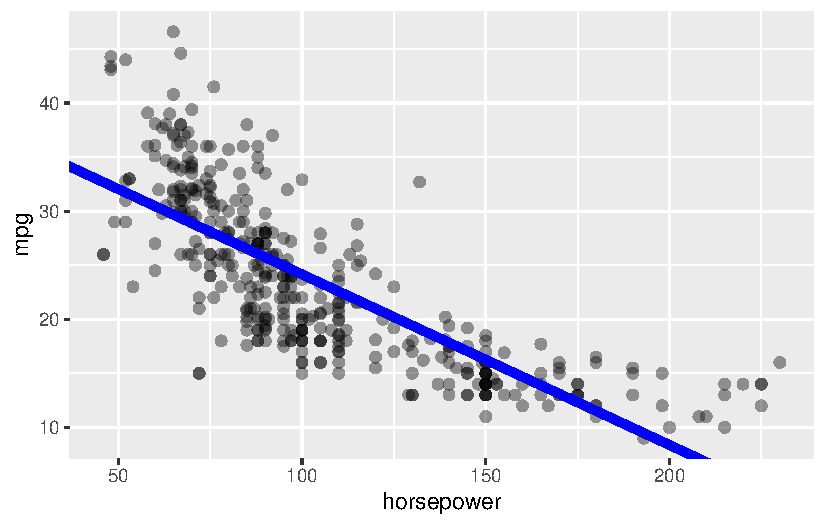
\includegraphics{HW-9-Linear-Regression_files/figure-pdf/unnamed-chunk-6-1.pdf}

}

\end{figure}

\hypertarget{c-use-the-plot-function-to-produce-diagnostic-plots-of-the-least-squares-regression-fit.-comment-on-any-problems-you-see-with-the-fit.}{%
\subparagraph{c) Use the plot() function to produce diagnostic plots of
the least squares regression fit. Comment on any problems you see with
the
fit.}\label{c-use-the-plot-function-to-produce-diagnostic-plots-of-the-least-squares-regression-fit.-comment-on-any-problems-you-see-with-the-fit.}}

\begin{Shaded}
\begin{Highlighting}[]
\NormalTok{linearmodelauto }\SpecialCharTok{\%\textgreater{}\%}\NormalTok{ performance}\SpecialCharTok{::}\FunctionTok{check\_model}\NormalTok{()}
\end{Highlighting}
\end{Shaded}

\begin{figure}[H]

{\centering 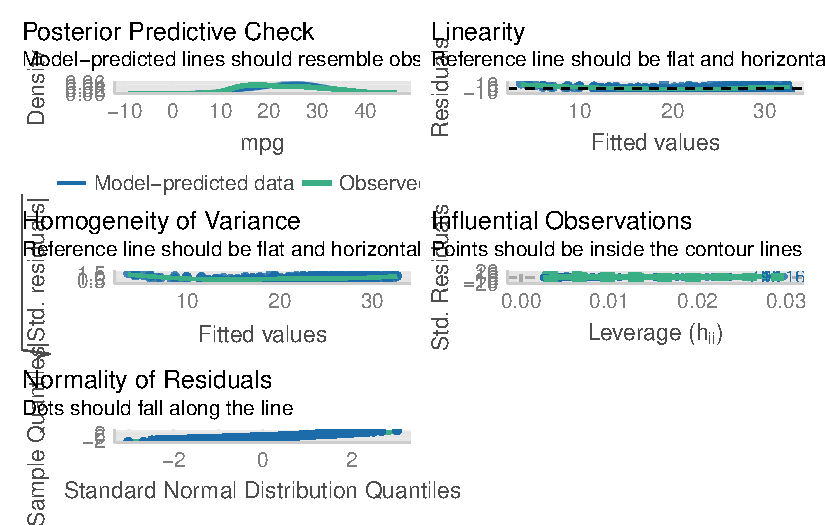
\includegraphics{HW-9-Linear-Regression_files/figure-pdf/unnamed-chunk-7-1.pdf}

}

\end{figure}

\hypertarget{section-1}{%
\subparagraph{~}\label{section-1}}



\end{document}
